\documentclass{scrartcl}
\usepackage{graphicx}
\usepackage{multicol}
\raggedright
\begin{document}

\title{Exploring genetic data from the Human Genome Diversity Project}
\subtitle{Data Science 2 Project Proposal}
\author{Nick Strayer}
\date{\today} 
\maketitle

{ \Large Introduction}
\vspace{.7em}

The world of genetics is a fantastically exciting one. Over the past decades our understanding and technology to obtain genetic information has ballooned. Genetic data, especially with the advent of full genome sequencing, is growing faster than Moore's law[1]. Researchers in the computational sciences have always been fairly blessed by the relentless advancement of computing power, now here we are back in the ages of needing to develop new methods of analyzing at data rather than simply waiting for the computer to be fast enough to do it for us. 
\vspace{0.5em}

Another facet of genetic data that appeals to me is it's ability to give us a new lens upon which to view society. We live in a world where judgements are made on the qualitative. "His skin is darker than mine, therefor X." As humans we are programed from our roots as tribe based hunter gatherers to dislike those that don't look or act like us, back then it was a matter of survival. Today life or death is no longer dependent upon the success of a hunt or the fertility of the soil any given month and thus our tribal lifestyles have vanished. From an evolutionary point of view this massive change in lifestyle was a mere blink of the eye, as a result we live in a modern society burdened by the identification methods of our tribal ancestors. Genetic data offers an unprecedented opportunity to see the world in a new light. One not of qualitative differences such as skin color but as quantitative differences in the building blocks of life. 
\vspace{0.5em}

In 2007 researchers at Stanford University began an effort to explore the genetic differences between populations of the world. They analyzed the DNA of 1,043 individuals from different locations all around the world. For each of these individuals they looked at more than 650,000 single-nucleotide polymorphism (SNP) markers(figure 1).  SNPs are linked pairs of the basic building blocks of DNA, Adenine(A), Thymine(T), Cytosine(C) and Guanine(G). The different combinations of these nucleobases form the programing language of biology. The info they contain is read by the cell and then used to make different proteins that compose you (or whatever thing the DNA belongs to). There are many billions of these pairings on a single strand of DNA but huge proportions of them are the same between people, or even between totally different things (for example, 50\% of these pair or nucleobases is identical between humans and bananas.) Because of this fact (and the cost of sequencing) the Stanford project selected 660 thousand sites upon which to sequence. 

\begin{figure}[h!]
  \caption{Explanation of SNPs}
  \centering
   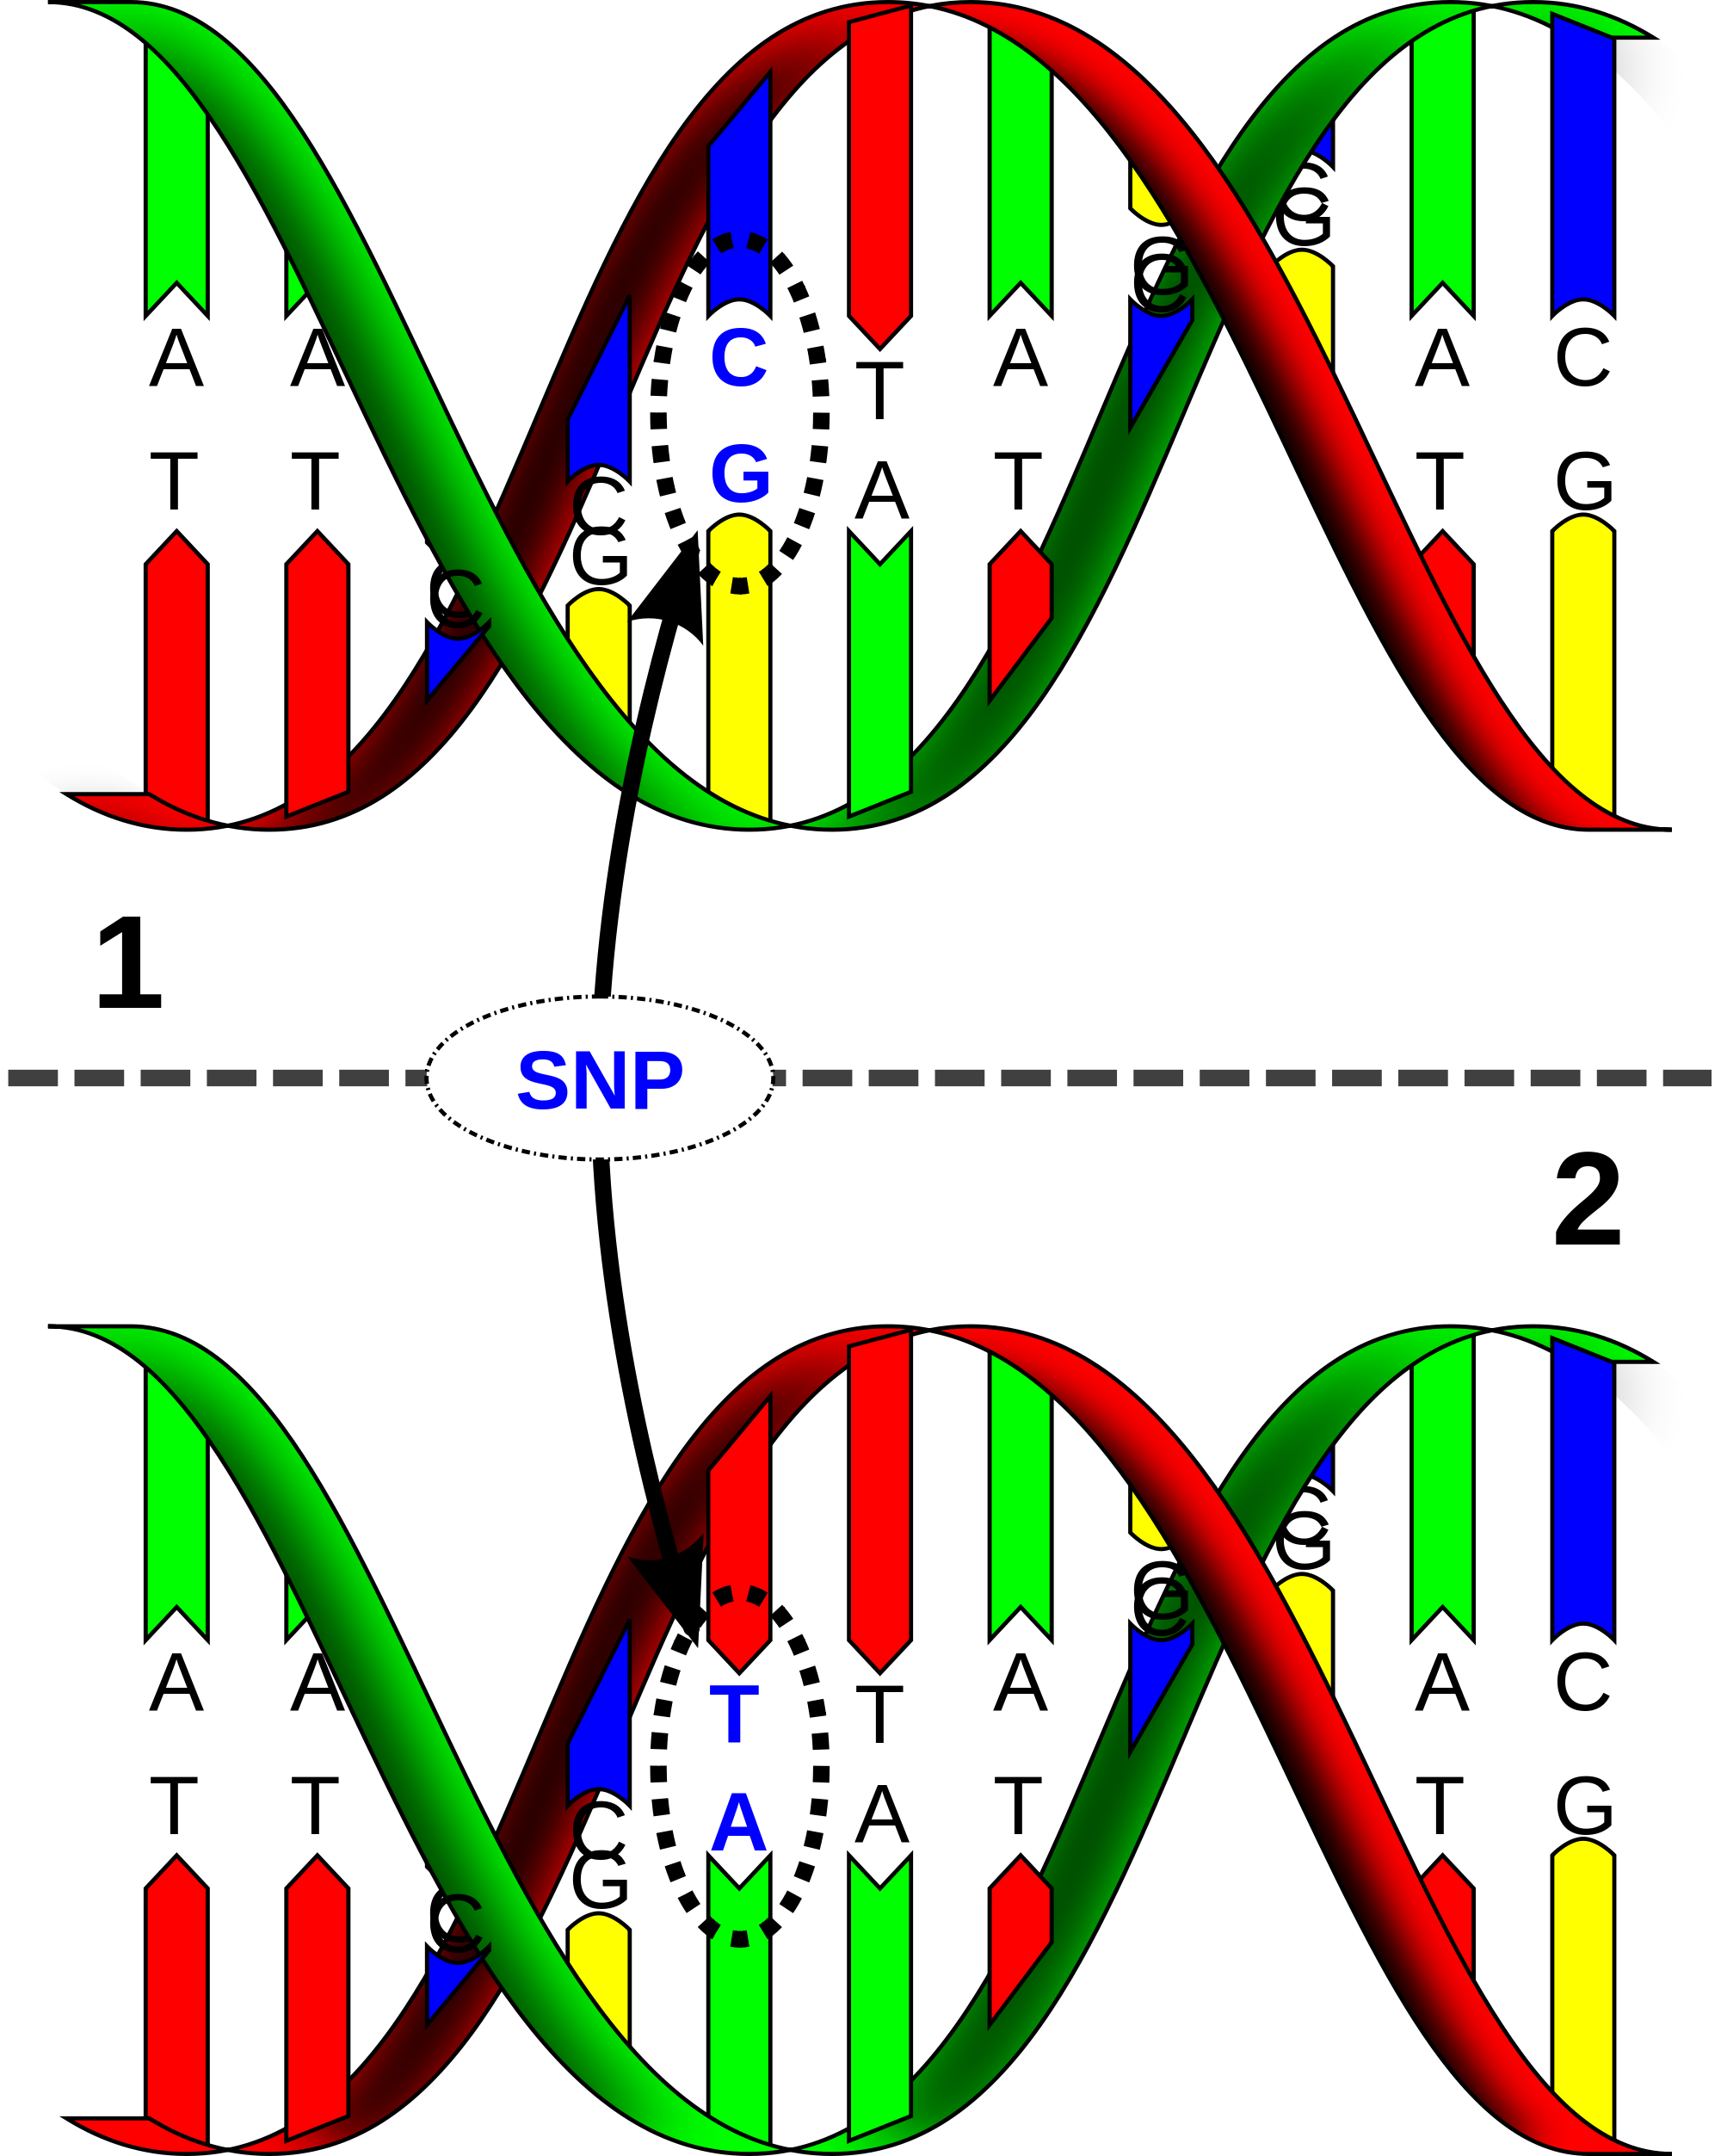
\includegraphics[scale = .06]{figures/snp_explanation.png}
\end{figure}

{\Large What I will do:}
\vspace{.7em}

I will take the raw data from the HGDP dataset (which is in the form 1043 columns of individuals with 650 thousand rows of the different SNPs,) and test multiple hypotheses that various different alleles are more frequent (figure 2) in different populations (e.g. central african, north american). 
\vspace{0.5em}

\begin{figure}[h!]
  \caption{Sample data output}
  \centering
   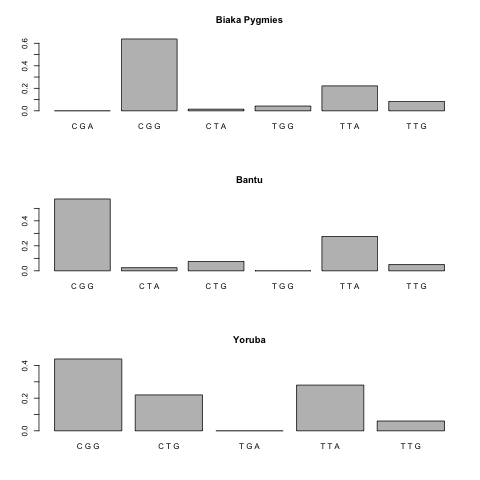
\includegraphics[scale = .41]{figures/frequencyChart.png}
\end{figure}

I will cite previous literature in deciding which SNPs to test. For example, Ploomin et al 2006 identifies multiple loci upon which they believe (in small scale tests) there are strong links between intelligence and allele frequency. I am interested to see if any of these "trait genes" show geographic or tribal trends. If trends \textit{are} found, further digging into the results will be done. This could take the form of testing stereotypes empirically or seeing if there is correlation with any external population wide measures of that trait (such as test scores or graduate rates for intelligence.) 


\vspace{1em}
{\Large How I will do it:}
\vspace{.7em}

I will wrangle the full dataset into the form shown below in figure 3 using Python(the figure is of a smaller subset of the full data) . From this cleaned dataset I will do all of my statistical analysis in R as it has much more robust statistical genetics packages than Python. If spacial plotting is necessary or the results are particularly compelling in interactive form I will develop visualizations in JavaScript/ D3. 

\begin{figure}[h!]
  \caption{Sample data output}
  \centering
   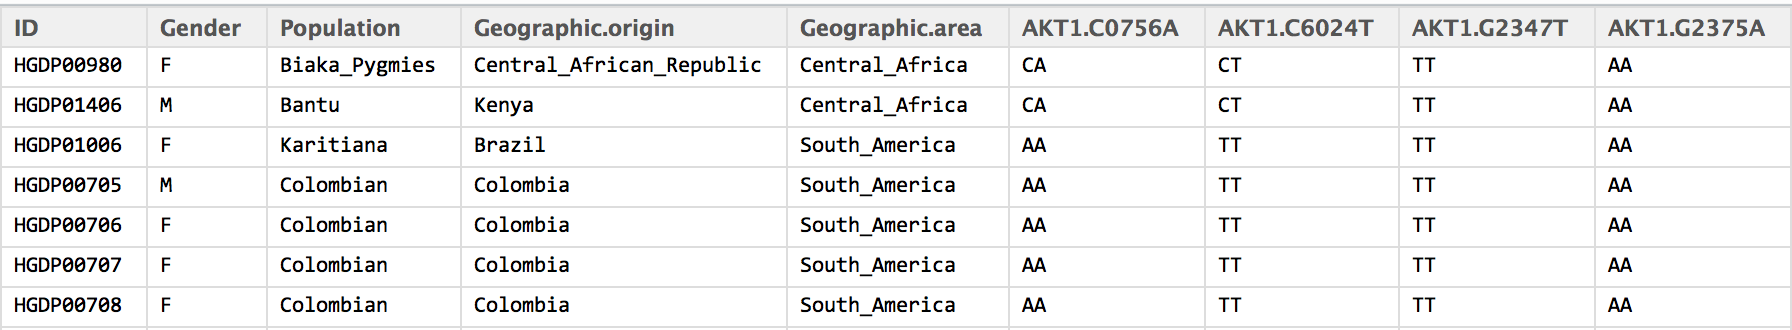
\includegraphics[scale = .5]{figures/sampleOutput.png}
\end{figure}

\vspace{1em}
{\Large Potential issues/ shortsightedness-es:}
\vspace{.7em}

I am very aware that genetics is very rarely, if ever, a binary issue. Almost always traits are much more complicated than a single base pair of DNA being present or not. My proposed approach does not take that into account. I have done this because research into these issues taking into account the multi-local nature of genetic roots of traits is an ongoing field with many very smart people working at the issue. If I took it on from the start I would almost assuredly spend the rest of the semester getting nothing of value. 
\vspace{.5em}

That being said, depending on the productivity and success of the previously stated single-loci objectives I could potentially attempt to tackle the complex nature. My first thoughts on doing so are to use a machine learning algorithm hooked up to an arbitrary number of snps and to assign a trait "score" to a given population based upon external data (crazy amounts of assumption), then see how well the algorithm does (using a training set of only 521 individuals) at predicting that score. This approach would be much more valuable on genetic data for say, cancer patients. 




\vspace{10em}
{\Large Citations}
\begin{enumerate}
\item DNA Sequencing Caught in Deluge of Data, A. Pollack, New York Times, 2011,
http://www.nytimes.com/2011/12/01/business/dna-sequencing-caught-in-deluge-of-data.html

\item The quest for quantitative trait loci associated with intelligence, Robert Plomin, Joanna K.J. Kennedy, Ian W. Craig, Intelligence, Volume 34, Issue 6, November–December 2006, Pages 513 - 526

\end{enumerate}
\end{document}